\documentclass[a4paper,10pt]{article}
\usepackage[T1]{fontenc}
\usepackage[utf8]{inputenc}
\usepackage{amsmath}
\usepackage{graphicx}
\usepackage{titlepic}
\usepackage{url}
\usepackage[table,xcdraw]{xcolor}

\title{XLI OLIMPIADA GEOGRAFICZNA 2014/2015 SPOŁECZNO-GOSPODARCZE UWARUNKOWANIA ROZWOJU GMINY KIWITY I GMINY LUBOMINO}
\author{Łukasz Karczewski}

\begin{document}

\maketitle
\newpage
\tableofcontents
\newpage

\section{Wstęp}
  Gmina jest podstawową jednostką samorządu terytorialnego w Polsce. 
  Stopień rozwoju gmin jest jednym z wykładników rozwoju większych jednostek administracyjnych : powiatów i województw. 
  Bardzo często jednak w ocenie osiągniętego postępu gospodarczego wymienia się inwestycje głównych miast w Polsce. 
  Tymczasem progres w tej najmniejszej skali jest dużo ważniejszy dla obywateli, ponieważ dotyczy ich codziennych problemów.
  Warto przyjrzeć się uwarunkowaniom rozwoju w najsłabiej rozwiniętym regionie Polski : województwie warmińsko-mazurskim. 
  Województwo te nie ma rozwiniętego przemysłu i bazy surowcowej, co czyni je nieatrakcyjnym na rynku pracy. 
  Rolnictwo oraz branża usług i turystyki mimo dużego potencjału wciąż pozostają niedofinansowanie i przez to niekonkurencyjne w skali krajowej. 
  Od przystąpienia Polski do Unii Europejskiej w 2004 roku jednostki samorządu terytorialnego dzięki dotacjom starają się zmienić ten niekorzystny obraz 
  i zaczynają wykorzystywać potencjał swojego regionu.
\section{Uzasadnienie wyboru gmin}
  Głównym kryterium wyboru Gmin Kiwity i Lubomino było ich podobieństwo na płaszczyźnie administracyjnej, demograficznej, gospodarczej i komunikacyjnej. 
  Są to gminy wiejskie leżące w tym samym województwie i powiecie, o zbliżonej liczbie ludności i powierzchni oraz gospodarce opierającej się głównie na rolnictwie. 
  Z uwagi na to, że są położone w tej samej jednostce administracyjnej można porównać operatywność miejscowych działaczy, 
  którzy mają do dyspozycji podobne środki ze wspólnego źródła, jakim są finanse województwa.
  
\newpage
\section{Ogólna charakterystyka gospodarek wybranych gmin}
  \subsection{Społeczno-gospodarcza charakterystyka gminy Kiwity}
    Gmina Kiwity położona jest w powiecie lidzbarskim w północnej części  województwa warmińsko–mazurskiego. 
    Graniczy ona z gminami: od zachodu –Lidzbark Warmiński, od północy - Bartoszyce, od wschodu – Bisztynek, od południa – Jeziorany (Mapa 1).
    \begin{figure}[!htb]
    \centering
	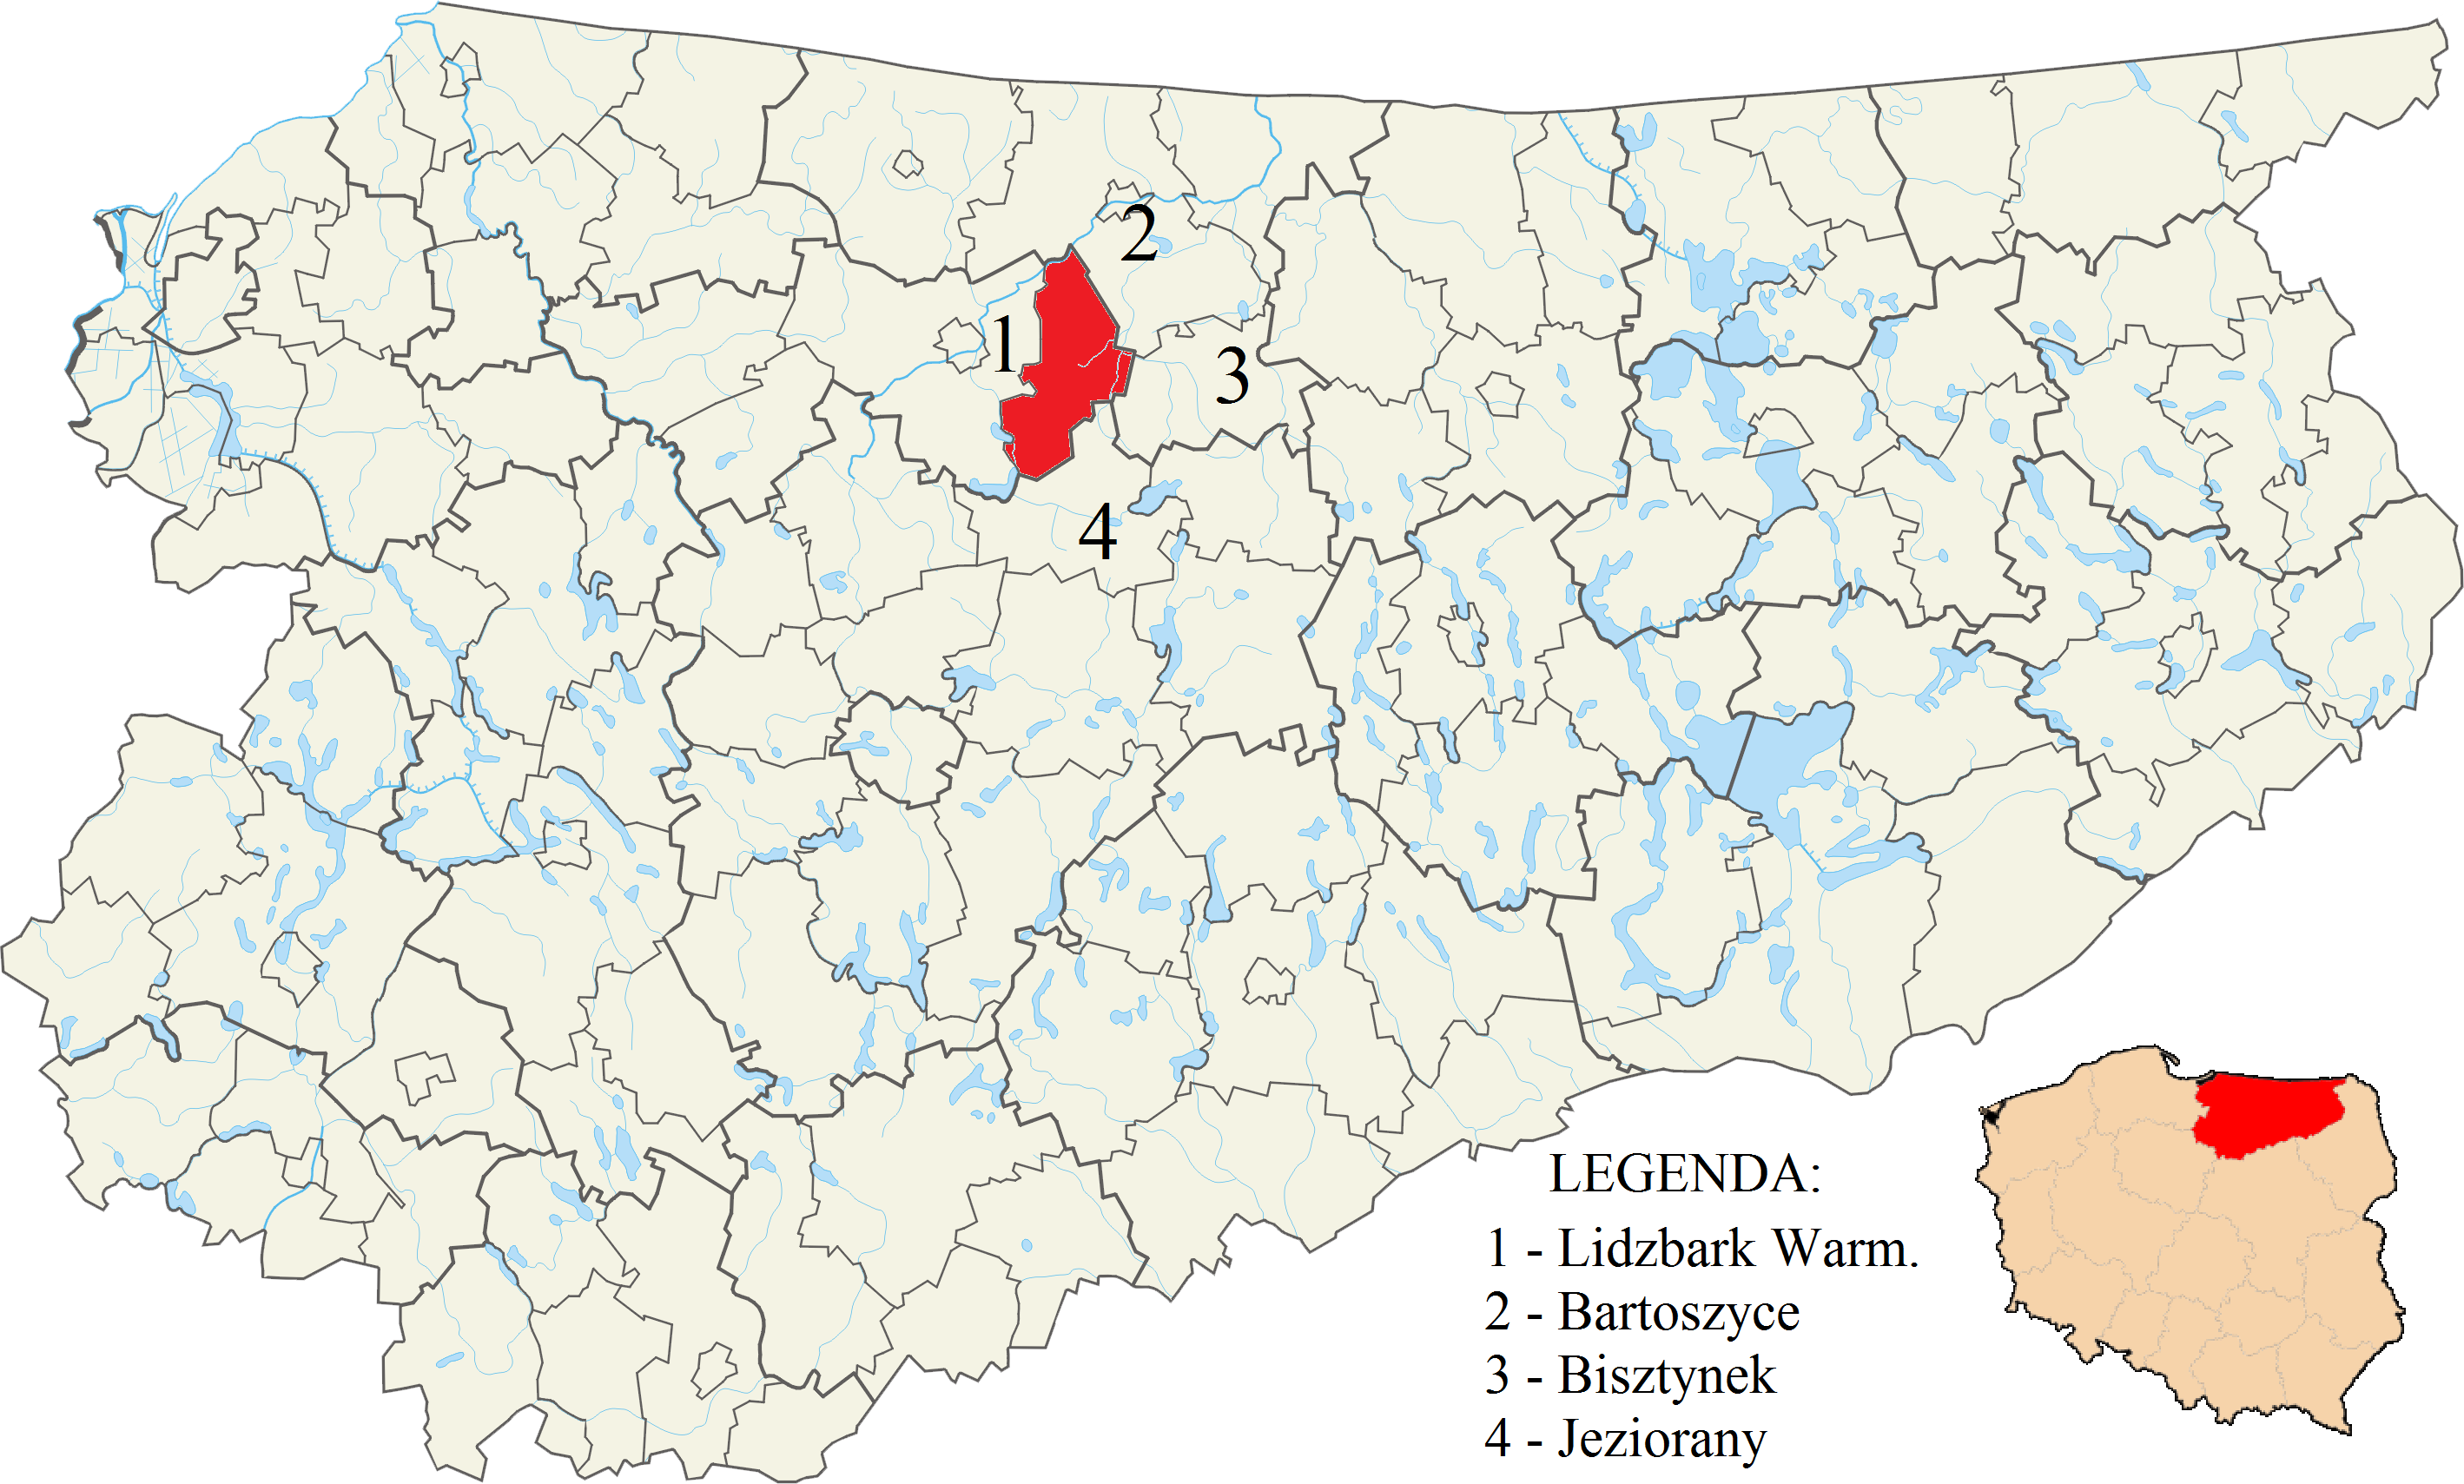
\includegraphics[scale=0.12]{pics/mapa1.png}
	\caption{Lokalizacja gminy Kiwity w województwie warmińsko-mazurskim}
    \end{figure}
    Powierzchnia gminy wynosi ok. 145 km2. Jej powierzchnia stanowi 0,6\% powierzchni województwa i 18\% powierzchni powiatu. Użytki rolne stanowią ponad 75\% areału. 
    Pozostałe 15\% stanowią tereny leśne. Jest to gmina typowo rolnicza o wysokim potencjale przyrodniczym do produkcji rolnej.
    Według danych GUS z 2012 roku, gminę zamieszkiwało 3417 osób, a gęstość zaludnienia wynosiła 24 osoby na $1 km^{2}$.
    Najważniejsze walory przyrodniczo-krajobrazowe stanowią tereny Użytku Ekologicznego Bartniki z uwagi na miejsca lęgowe wielu rzadkich gatunków ptaków (Zdjęcie 1).
    \begin{figure}[!htb]
    \centering
	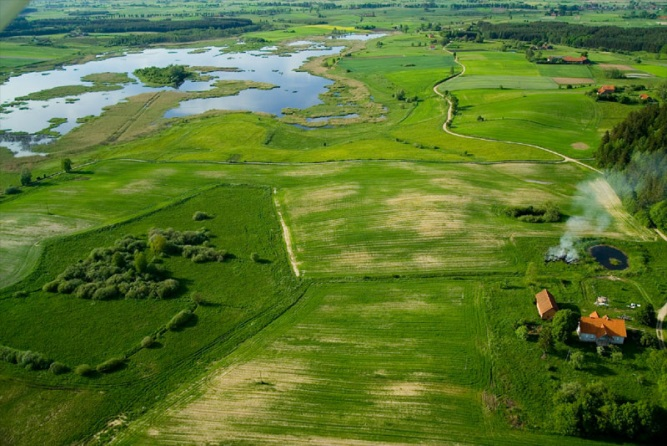
\includegraphics{pics/zdjecie1.jpg}
	\caption{Użytek ekologiczny Bartniki}
    \end{figure}
    
    Najciekawszą atrakcją turystyczną gminy jest Bazylika Nawiedzenia Najświętszej Maryi Panny w Stoczku Klasztornym, odwiedzana przez turystów z Polski i Europy (Zdjęcie 2).
    \begin{figure}[!htb]
    \centering
	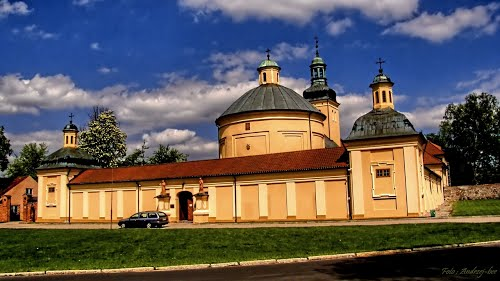
\includegraphics[scale=0.5]{pics/zdjecie2.jpg}
	\caption{Bazylika Nawiedzenia Najświętszej Maryi Panny w Stoczku Klasztornym}
    \end{figure}
    
    Gmina połączona jest z miastem Bartoszyce oraz przejściem granicznym w Bezledach drogą krajową nr 51. 
    Droga krajowa i  wojewódzka nr 513 łączy gminę z Lidzbarkiem Warmińskim. Droga ta stanowi nadrzędny układ komunikacyjny wiążący gminę z układem dróg szybkiego ruchu. 
    Pozostałe drogi w gminie to drogi powiatowe i gminne, które wiążą miejscowości z ośrodkami usługowymi rozmieszczonymi na jej terenie (Mapa 2).
    \begin{figure}[!htb]
    \centering
	\includegraphics[scale=0.1]{pics/mapa2.jpg}
	\caption{Obszar gminy Kiwity}
    \end{figure}
    \newpage
    W Gminie Kiwity pracujących jest 138 osób. Liczba zarejestrowanych osób bezrobotnych wynosi 265 co stanowi 11,8\% ludności w wieku produkcyjnym. 
    Pozostała część ludności zajmuje się rolnictwem.W dotychczasowym rozwoju gminy główna funkcją gospodarczą i źródłem utrzymania ludności było rolnictwo. 
    Na obszarze gminy położonych jest około 500 gospodarstw. W ostatnich latach rozwinęła się przedsiębiorczość i drobne zakłady usługowo-produkcyjne. 
    Na terenie Gminy Kiwity są zarejestrowane 142 firmy . Są to firmy działające w sektorze rolniczym, przemysłowym i budowlanym. 
    Największymi podmiotami gospodarczymi w gminie są F.H.U. „Stemar” oraz F.H.U. „Animar”. 
    Firmy te zajmują się działalnością handlowo-usługową, głównie sprzedażą artykułów budowlanych oraz skupem zboża.
  \subsection{Społeczno-gospodarcza charakterystyka gminy Lubomino}
    Gmina Lubomino jest gminą położoną w północnej części województwa warmińsko-mazurskiego. 
    Graniczy z gminami: Orneta, Lidzbark Warmiński, Dobre Miasto, Świątki oraz Miłakowo (Mapa 3).
    
    \begin{figure}[!htb]
    \centering
	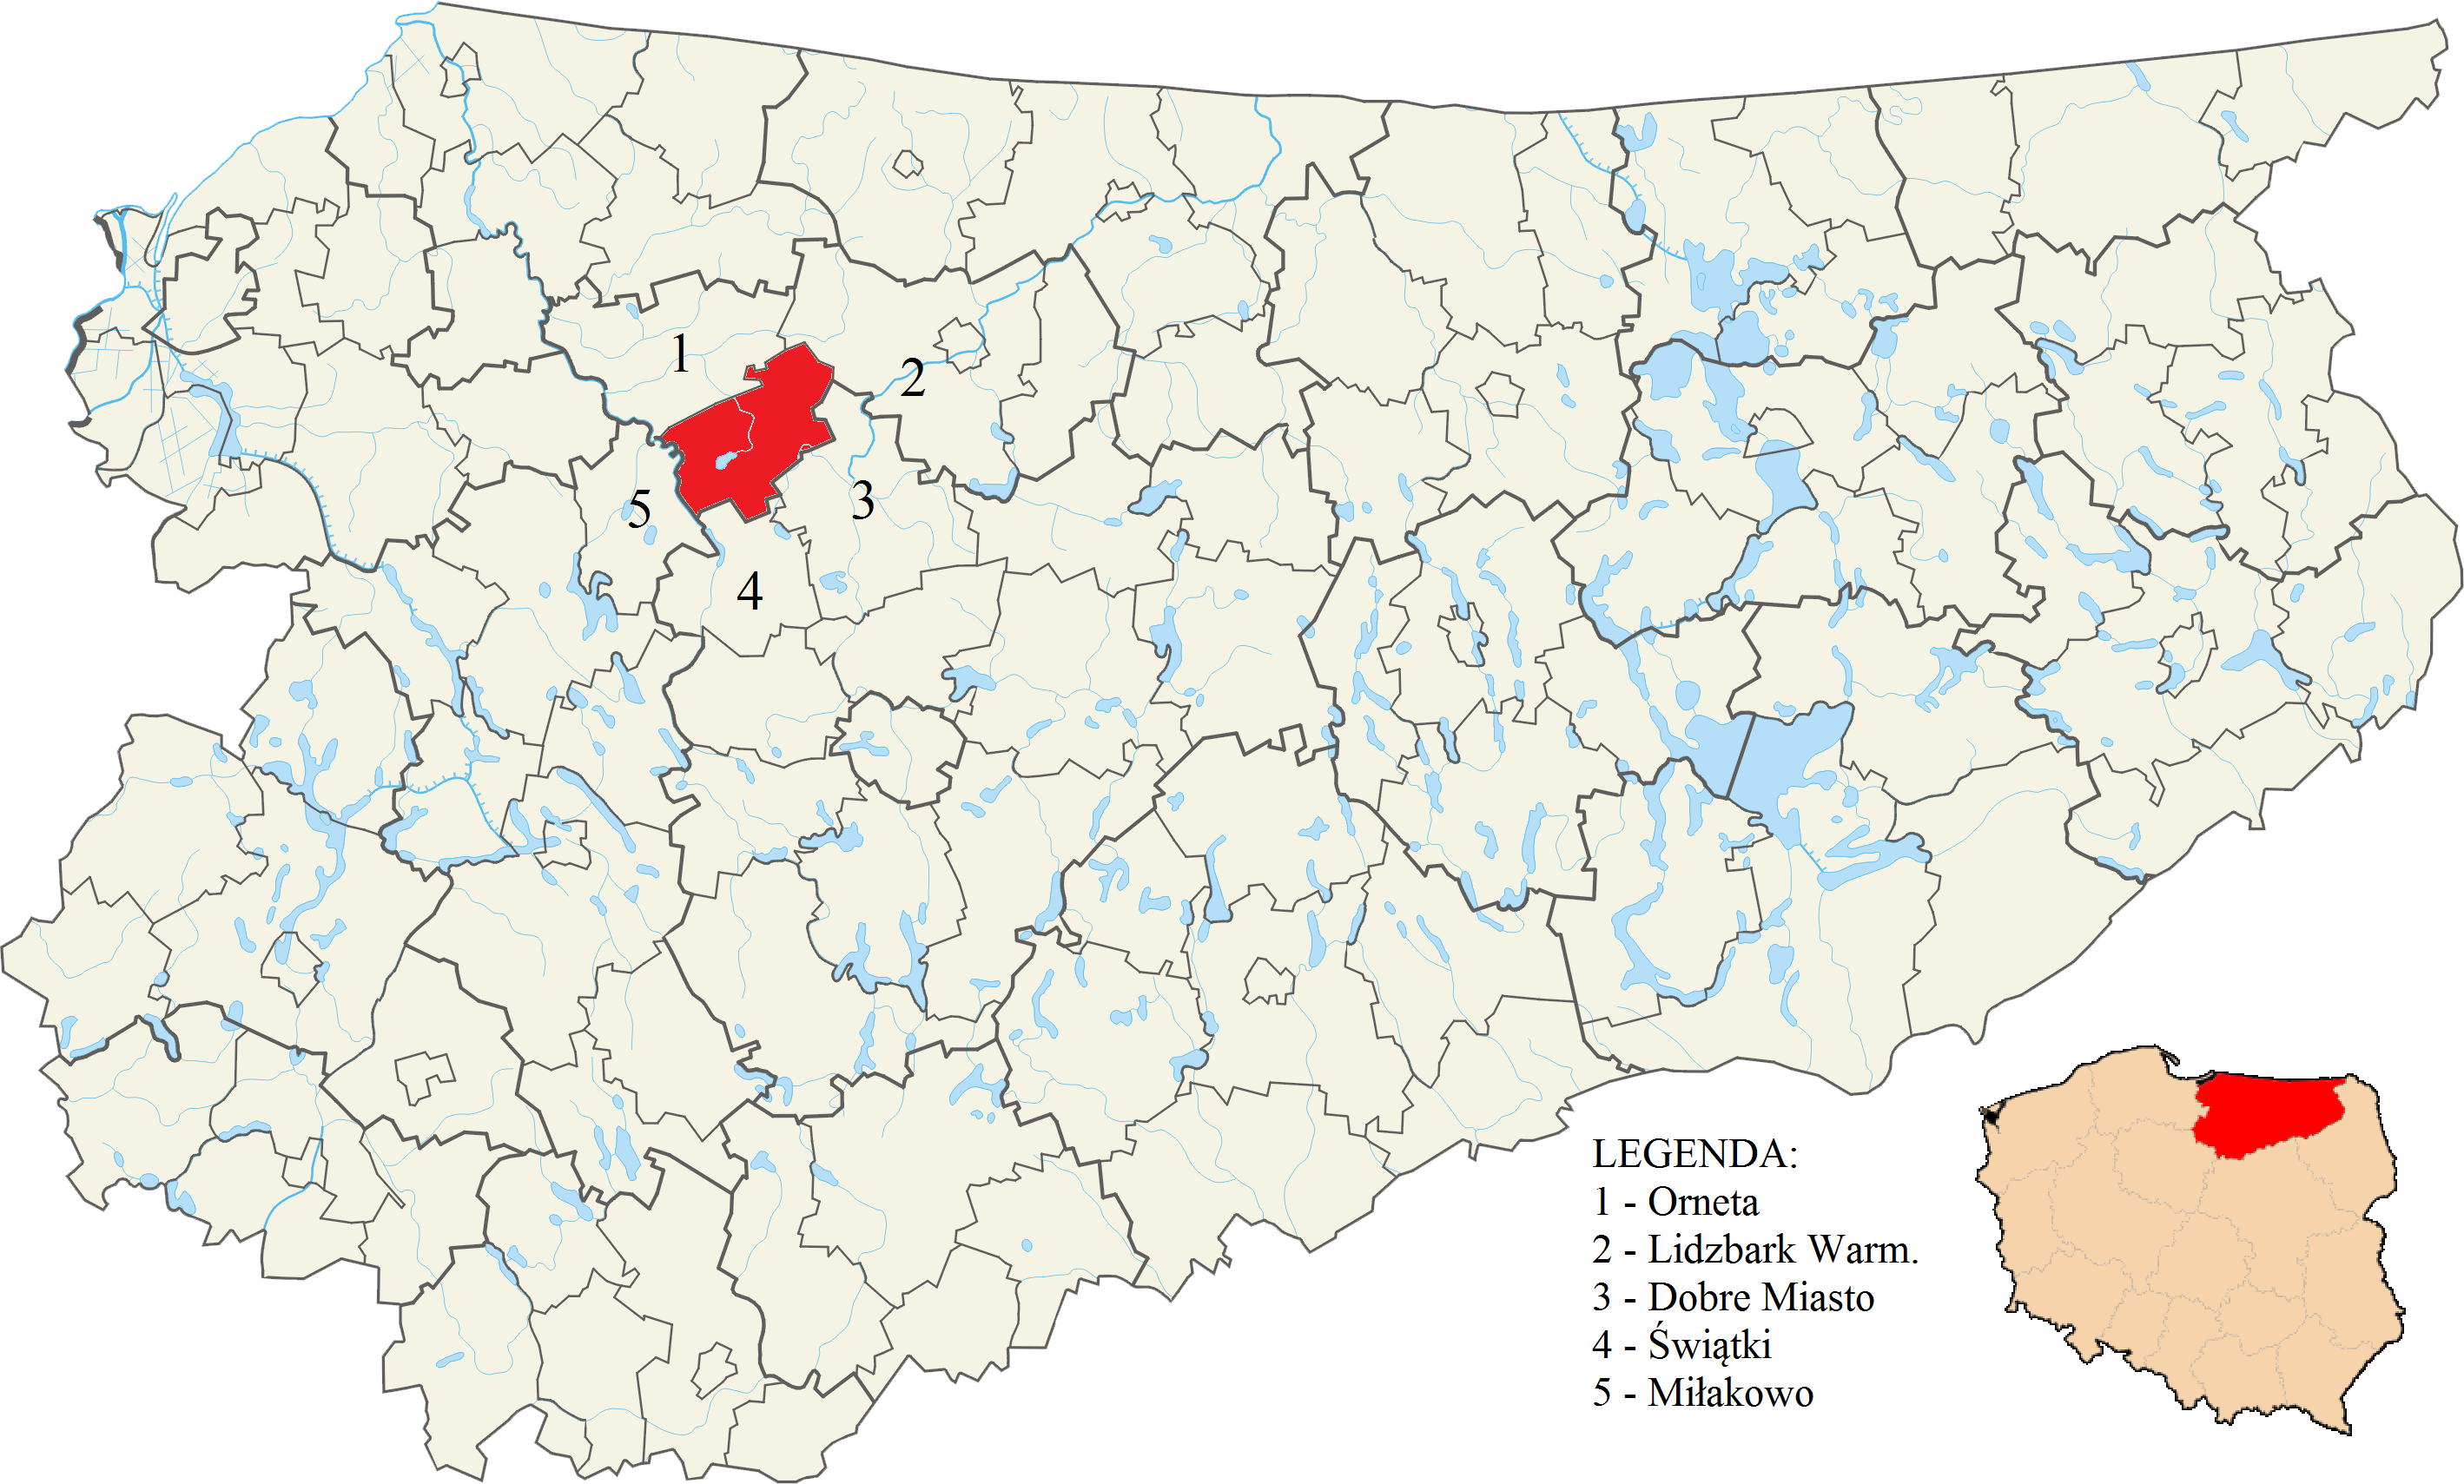
\includegraphics[scale=0.12]{pics/mapa3.png}
	\caption{Lokalizacja gminy Lubomino w województwie warmińsko-mazurskim}
    \end{figure}
    Główny Urząd Statystyczny podaje, że w 2012 roku ludność gminy wynosiła 3659 osób. Gęstość zaludnienia wynosiła 24 osoby na $1 km^{2}$.
    Powierzchnia gminy to około 149 km2. Użytki rolne stanowią ok. 82\% powierzchni gminy. Pozostałe 18\% to tereny leśne. 
    Jest to gmina o profilu rolniczym z elementami przemysłu.
    Główną atrakcją turystyczno-przyrodniczą gminy jest Jezioro Tonka o powierzchni 162 ha (Zdjęcie 3).
    
    \begin{figure}[!htb]
    \centering
	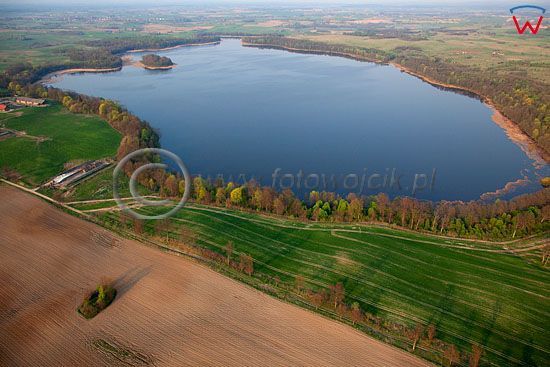
\includegraphics[scale=0.5]{pics/zdjecie3.jpg}
	\caption{Jezioro Tonka}
    \end{figure}
    \newpage
    Gmina Lubomino jest bezpośrednio połączona z miastami Orneta i Dobre Miasto drogą krajową nr 507. Drogi wewnętrzne stanowią połączenia między wioskami wewnątrz gminy. 
    Na terenie gminy są dwa przystanki kolejowe: w Lubominie i Rogiedlach, wraz z bocznicami. 
    Połączenie kolejowe wykorzystywane jest przez osoby dojeżdżające do Olsztyna i Dobrego Miasta (Mapa 4).
    W Gminie Lubomino pracujących jest 214 osób. Zarejestrowane bezrobocie wynosi 16,3\%. 
    Pozostała część ludności zajmuje się rolnictwem. Na terenie gminy położonych jest 507 indywidualnych gospodarstw rolnych.
    Wśród 193 zarejestrowanych podmiotów gospodarczych z sektora rolniczego, przemysłowego i budowlanego największymi są F.H.U. „Lemar” oraz Przedsiębiorstwo Produkcyjne „Siat-Tom”. 
    F.H.U. „Lemar” zajmuje się sprzedażą drewna i węgla, natomiast Przedsiębiorstwo Produkcyjne „Siat-Tom” wytwarza gotowe wyroby metalowe.
    \begin{figure}[!htb]
    \centering
	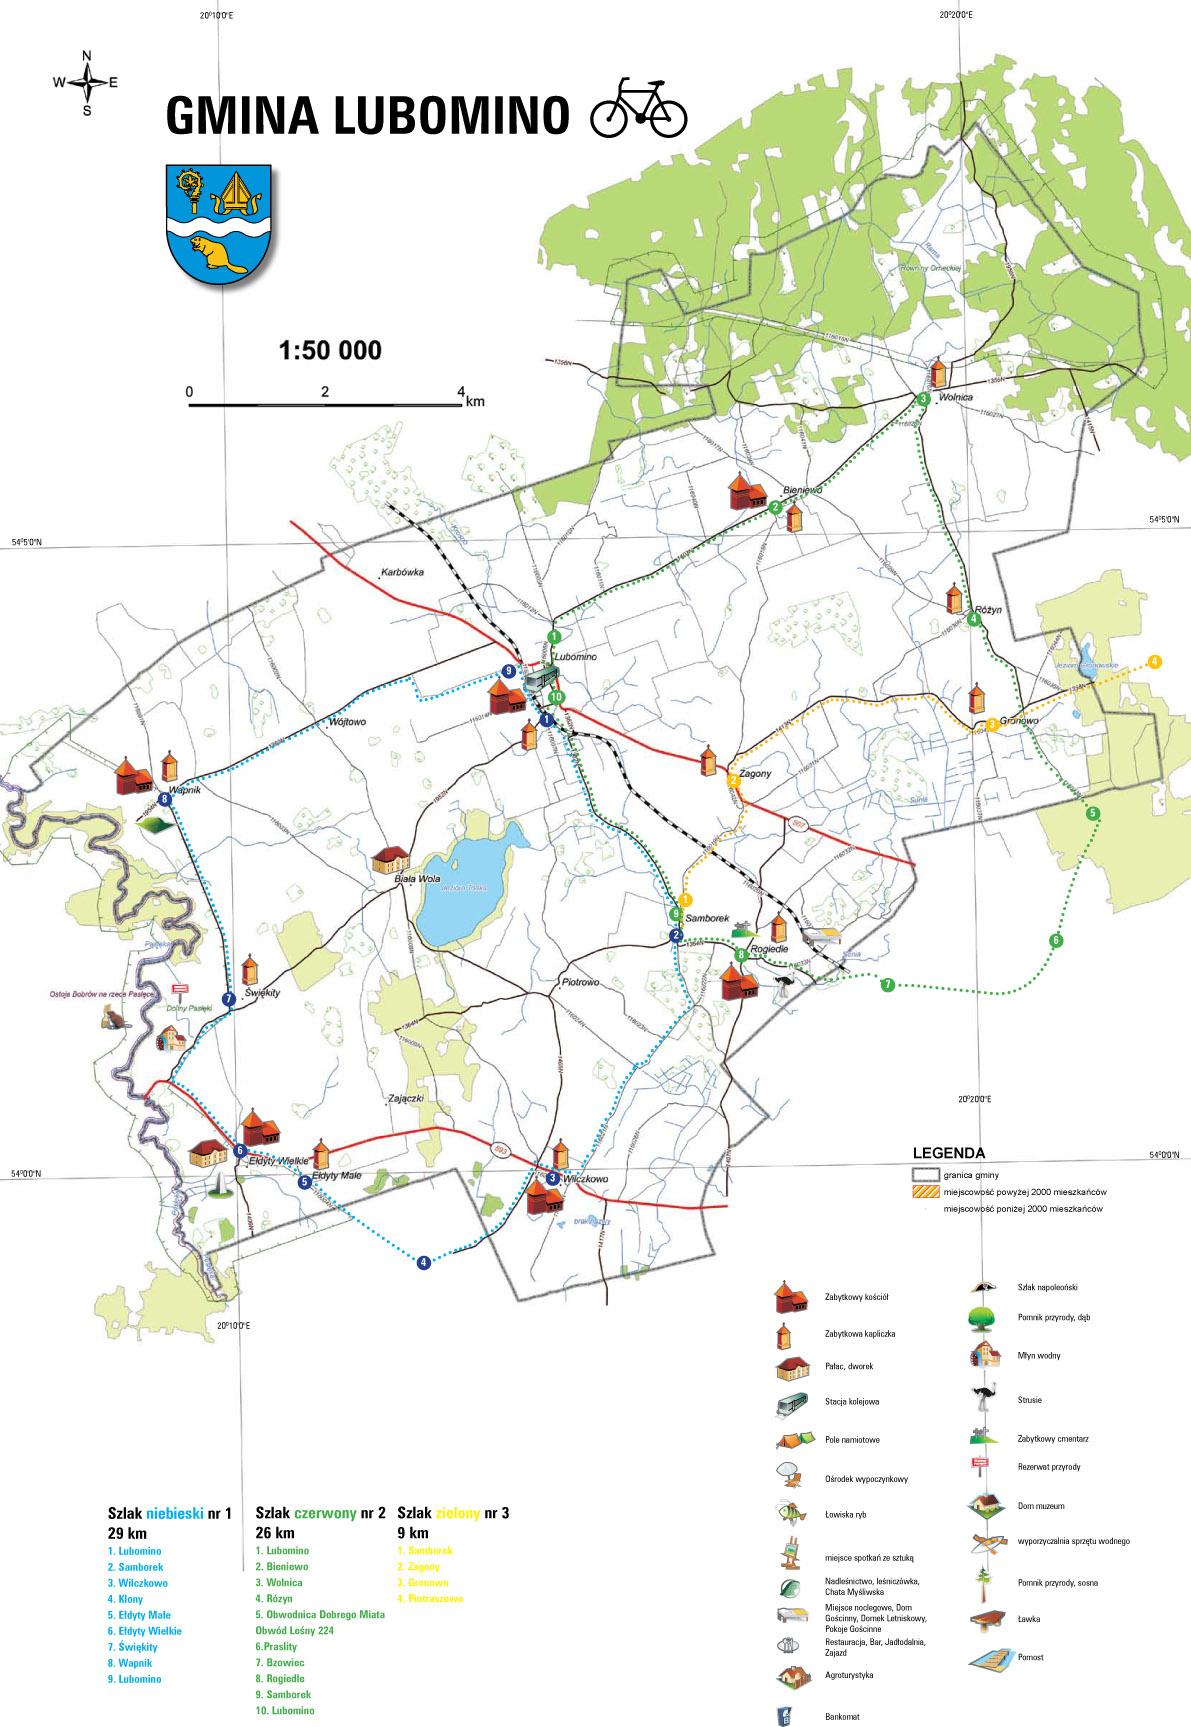
\includegraphics[scale=0.2]{pics/mapa4.jpg}
	\caption{Obszar gminy Lubomino}
    \end{figure}
    
\section{Budżety wybranych gmin}
  \subsection{Budżet gminy Kiwity}
    
    Deficyt budżetu gminy wynosi 1 923 877 zł. 
    Zostanie pokryty przychodami pochodzącymi z wolnych środków w wysokości 1 680 000 zł, 
    nadwyżki budżetu jednostki samorządu terytorialnego z lat ubiegłych w wysokości 11 623 zł, oraz kredytów w wysokości 232 254 zł.
    Planuje się uzyskać środki z Funduszu Spójności oraz innych funduszy strukturalnych Unii Europejskiej na realizację inwestycji w gminie na kwotę 652 636 zł.
    
    \begin{table}[!htb]
    \centering
    \caption{Dochody budżetu gminy Kiwity}
    \label{my-label}
    \begin{tabular}{llllllll}
    \multicolumn{8}{c}{\cellcolor[HTML]{3166FF}{\color[HTML]{FFFFFF} DOCHODY}}                 \\
    \multicolumn{7}{l}{\textbf{Dochody bierzące}}                 & \textbf{10 044 303 zł}     \\
       & \multicolumn{6}{l}{Dochody własne}                   & 4 182 191 zł               \\
       & \multicolumn{6}{l}{Subwencja ogólna}                 & 4 203 526 zł               \\ 
       & \multicolumn{6}{l}{Dotacje z budżetu państwa}        & 1 757 086 zł               \\
    \multicolumn{7}{l}{\textbf{Dochody majątkowe}}                & \textbf{751 136 zł}        \\
    \multicolumn{8}{r}{\cellcolor[HTML]{3166FF}{\color[HTML]{FFFFFF} ŁĄCZNIE : 10 757 439 zł}}
    \end{tabular}
    \end{table}
    
    \begin{table}[!htb]
    \centering
    \caption{Wydatki budżetu gminy Kiwity}
    \label{my-label}
    \begin{tabular}{lllllll}
    \multicolumn{7}{c}{\cellcolor[HTML]{3166FF}{\color[HTML]{FFFFFF} \textbf{WYDATKI}}}                \\
    \textbf{Wydatki bierzące}              & \multicolumn{6}{l}{\textbf{10 470 998 zł}}                \\
    \textbf{Wydatki inwestycyjne}          & \multicolumn{6}{l}{\textbf{2 248 318 zł}}                 \\
    \textbf{Wydatki majątkowe}             & \multicolumn{6}{l}{\textbf{1 339 962 zł}}                 \\
    \multicolumn{7}{r}{\cellcolor[HTML]{3166FF}{\color[HTML]{FFFFFF} \textbf{ŁĄCZNIE: 12 719 316 zł}}}
    \end{tabular}
    \end{table}
    
  \subsection{Budżet gminy Lubomino}
  
    Deficyt budżetu gminy wynosi 248 405 zł i zostanie pokryty przychodami z zaciągniętego kredytu i pożyczki.
    Planuje się uzyskać środki z Funduszu Spójności oraz innych funduszy strukturalnych Unii Europejskiej na realizację inwestycji w gminie na kwotę 625 378 zł.
    
    \begin{table}[!htb]
    \centering
    \caption{Dochody budżetu gminy Lubomino}
    \label{my-label}
    \begin{tabular}{llllllll}
    \multicolumn{8}{c}{\cellcolor[HTML]{3166FF}{\color[HTML]{FFFFFF} DOCHODY}}                 \\
    \multicolumn{7}{l}{\textbf{Dochody bierzące}}                 & \textbf{10 615 521 zł}     \\
       & \multicolumn{6}{l}{Dochody własne}                   & 4 024 613 zł               \\
       & \multicolumn{6}{l}{Subwencja ogólna}                 & 4 215 692 zł               \\ 
       & \multicolumn{6}{l}{Dotacje z budżetu państwa}        & 2 375 216 zł               \\
    \multicolumn{7}{l}{\textbf{Dochody majątkowe}}                & \textbf{1 313 781 zł}        \\
    \multicolumn{8}{r}{\cellcolor[HTML]{3166FF}{\color[HTML]{FFFFFF} ŁĄCZNIE : 11 929 302 zł}}
    \end{tabular}
    \end{table}
    
    \begin{table}[!htb]
    \centering
    \caption{Wydatki budżetu gminy Lubomino}
    \label{my-label}
    \begin{tabular}{lllllll}
    \multicolumn{7}{c}{\cellcolor[HTML]{3166FF}{\color[HTML]{FFFFFF} \textbf{WYDATKI}}}                \\
    \textbf{Wydatki bierzące}              & \multicolumn{6}{l}{\textbf{10 615 521 zł}}                \\
    \textbf{Wydatki inwestycyjne}          & \multicolumn{6}{l}{\textbf{1 562 186 zł}}                 \\
    \textbf{Wydatki majątkowe}             & \multicolumn{6}{l}{\textbf{1 532 186 zł}}                 \\
    \multicolumn{7}{r}{\cellcolor[HTML]{3166FF}{\color[HTML]{FFFFFF} \textbf{ŁĄCZNIE: 12 177 707 zł}}}
    \end{tabular}
    \end{table}
  
  \subsection{Porównanie budżetów gminy Kiwity i gminy Lubomino}
    Dochody gminy Lubomino są wyższe niż dochody gminy Kiwity. 
    Może wynikać to z większej ilości zarejestrowanych podmiotów gospodarczych, a przez to większych wpływów z podatków (Tabela 1 i Tabela 3).
    Wydatki gminy Kiwity nieznacznie przewyższają wydatki gminy Lubomino. 
    Jednakże przy niższe dochody co powodują również różnicę w deficytach budżetowych na niekorzyść gminy Kiwity. 
    W obydwu gminach deficyt zostanie pokryty przychodami z zaciągniętych kredytów i pożyczek (Tabela 2 i Tabela 4).
    Ilość środków, które planuje się pozyskać z funduszów Unii Europejskiej w obydwu gminach jest na zbliżonym poziomie.

\section{Bariery i czynniki rozwoju wybranych gmin}
  \subsection{Bariery i czynniki rozwoju gminy Kiwity}
    Czynniki rozwoju:
    
    \begin{itemize}
     \item Bardzo korzystne warunki przyrodniczo-rolnicze
     \item Dobrze prosperujące gospodarstwa rolne
     \item Połączenie z przejściem granicznym w Bezledach
     \item Niewielka odległość od miasta powiatowego (15 km)
     \item Rozwój przedsiębiorczości mieszkańców
     \item Obecność obiektów i terenów o walorach turystycznych (Użytek ekologiczny w Bartnikach, Bazylika w Stoczku Klasztornym)
     \item Walory przyrodniczo-krajobrazowe stwarzają warunki do rozwoju agroturystki
    \end{itemize}
    
    Bariery rozwojowe:
    \begin{itemize}
     \item Brak większych zakładów przemysłowych i przetwórczych na terenie gminy
     \item Brak bazy surowcowej dla rozwoju przemysłu
     \item Zły stan infrastruktury drogowej
     \item Rozproszenie osadnictwa
     \item Migracja osób wykształconych
     \item Wysoki odsetek osób korzystający z pomocy społecznej
     \item Niskie nakłady inwestycyjne
    \end{itemize}
    
    Najważniejszym czynnikiem rozwoju gminy są jej korzystne warunki przyrodniczo-rolnicze, które wpływają na zamożność mieszkańców, 
    których głównym zajęciem jest rolnictwo.
    Największą barierą rozwojową są niskie nakłady inwestycyjne, bez których gmina nie może się dynamicznie rozwijać. 
    Wynika to z wysokiego odsetka osób korzystających z pomocy społecznej, na którą wydawane jest więcej pieniędzy niż na inwestycje.
   
  \subsection{Bariery i czynniki rozwoju gminy Lubomino}
    Czynniki rozwoju:
    
    \begin{itemize}
     \item Bardzo korzystne warunki dla rozwoju rolnictwa
     \item Rozwijająca się przedsiębiorczość produkcyjna i usługowa
     \item Rozwinięta infrastruktura techniczno-ekonomiczna gminy
     \item Obecność linii kolejowej na terenie gminy
    \end{itemize}
    
    Bariery rozwojowe:
    \begin{itemize}
     \item Wysoki odsetek bezrobocia
     \item Duża liczba osób korzystająca z pomocy społecznej
     \item Migracja ludności wykształconej z terenu gminy
     \item Zły stan infrastruktury drogowej
     \item Niewielkie walory turystyczne
     \item Peryferyjne położenie gminy
     \item Niewielka ilość pieniędzy przeznaczona na inwestycje
    \end{itemize}
    
    Głównym czynnikiem rozwoju gminy jest rozwinięta infrastruktura techniczno-ekonomiczna, 
    która umożliwia rozwój lokalnych przedsiębiorstw oraz stwarza warunki do tworzenia nowych podmiotów gospodarczych.
    Największą barierą rozwojową niskie nakłady inwestycyjne, które mogłyby pomóc gminie w tempie jej rozwoju.

\newpage    
\section{Zakończenie}
  Przedstawione gminy posiadają duży potencjał rozwojowy. Jednakże małe nakłady inwestycyjne sprawiają, że nie jest on w pełni wykorzystywany. 
  Mogłaby temu zaradzić większa ilość projektów unijnych oraz otrzymywanych dotacji na rozwój infrastruktury oraz wspierania lokalnych przedsiębiorstw. 
  Takie działania uczyniłyby gminy atrakcyjniejsze dla nowych i obecnych mieszkańców oraz przedsiębiorców.
  Gmina Kiwity i gmina Lubomino powinny też zwiększyć wydatki na pomoc mieszkańcom w znajdowaniu zatrudnienia w gminie jak i poza nią. 
  Zmniejszyłoby to współczynnik bezrobocia, a przez to wydatki na pomoc społeczną, których część mogłaby być przeznaczona na rozwój gminy.

\newpage
\section{Bibliografia}
 \begin{itemize}
     \item Bański J.: Geografia polskiej wsi. PWE. Warszawa 2006
     \item Fierla I.: Geografia gospodarcza Polski. PWE. Warszawa 2004
     \item Fierla I.: Geografia gospodarcza Unii Europejskiej. PWE. Warszawa 2011
     \item Rogacki H.: Geografia społeczno-gospodarcza Polski. PWN. Warszawa 2007
     \item Czerny M.: Łuczak R., Makowski J., Globalistyka, PWN. Warszawa 2007
     \item Kondracki J.: Geografia regionalna Polski, PWN. Warszawa 2012
     \item Łęcki W.: Kanon krajoznawczy Polski. PTTK. Warszawa 2007
     \item Rocznik Statystyczny województw. GUS. Warszawa 2012
    \end{itemize}
\section{Wybrane wzory geograficzne}
  Poniższe wzory, mimo że nie mają kompletnie związku z pracą (może jeden), są powszechnie używane w geografii fizycznej, osadnictwa oraz ludności.
  \subsection{Współcznynnik spadku terenu pomiędzy dwoma punktami wyrażony w procentach}
  
   \begin{equation}
    S = \frac{\Delta h}{\Delta l} * 100\%
   \end{equation}
    
   Gdzie:
    
   $ S $ - współcznynnik spadku terenu
    
   $ \Delta h $ - różnica wysokości dwóch punktów
    
   $ \Delta l $ - odległość między dwoma punktami
    
  \subsection{Obliczanie wysokości górowania Słońca}
  
   \textbf{Dla dnia 22 czerwca (przesilenie letnie):}
    
   Półkula północna:
    
   \begin{equation}
    h = 90^{\circ} - \phi + 23^{\circ}{27}' 
   \end{equation}
    
   Półkula południowa:
    
   \begin{equation}
    h = 90^{\circ} - \phi - 23^{\circ}{27}' 
   \end{equation}

   \textbf{Dla dnia 22 grudnia (przesilenie zimowe):}
    
   Półkula północna:
    
   \begin{equation}
    h = 90^{\circ} - \phi - 23^{\circ}{27}' 
   \end{equation}
    
   Półkula południowa:
    
   \begin{equation}
    h = 90^{\circ} - \phi + 23^{\circ}{27}' 
   \end{equation}
     
   \textbf{Dla dnia 21 marca oraz 23 września (równonoc wiosenna i jesienna):}
    
   Dla obydwu półkul:
    
   \begin{equation}
    h = 90^{\circ} - \phi 
   \end{equation}
    
   \textbf{Gdzie:}
    
   $ h $ - wysokość górowania Słońca
    
   $ \phi $ - szerokość geograficzna punktu

  \subsection{Obliczanie bilansu wodnego}
  
  \begin{equation}
   P = HR + HP + E
  \end{equation}

  Gdzie:
  
  $ P $ - opad atmosferyczny
  
  $ HR $ - odpływ powierzchniowy(rzeczny) 
  
  $ HP $ - odpływ podziemny
  
  $ E $ - parowanie
  
  \subsection{Przyrost naturalny}
  
  \begin{equation}
   PN = U - Z
  \end{equation}
  
  Gdzie:
  
  $ PN $ - przyrost naturalny
  
  $ U $ - urodzenia
  
  $ Z $ - zgony

  \subsection{Współcznynnik przyrostu naturalnego}
  
  \begin{equation}
   W_{PN} = \frac{PN}{L}
  \end{equation}
  
  Gdzie:
  
  $ W_{PN} $ - współcznynnik przyrostu naturalnego
  
  $ PN $ - przyrost naturalny
  
  $ L $ - liczba ludności
    
  \subsection{Saldo migracji}
  
  \begin{equation}
   S_{M} = I - E
  \end{equation}

  Gdzie:
  
  $ S_{M} $ - saldo migracji
  
  $ I $ - liczba imigrantów
  
  $ E $ - liczba emigrantów
  
  \subsection{Przyrost rzeczywisty}
  
  \begin{equation}
   P_{R} = PN + S_{M}
  \end{equation}

  Gdzie:
  
  $ P_{R} $ - przyrost rzeczywisty
  
  $ PN $ - przyrost naturalny
  
  $ S_{M} $ - saldo migracji
  
  \subsection{Współcznynnik feminizacji}
  
  \begin{equation}
   W_{f} = \frac{K}{M} * 100
  \end{equation}
  
  Gdzie:
  
  $ W_{f} $ - współcznynnik feminizacji
  
  $ K $ - liczba kobiet
  
  $ M $ - liczba mężczyzn

  
  \subsection{Współcznynnik maskulinizacji}
  
  \begin{equation}
   W_{m} = \frac{M}{K} * 100
  \end{equation}

  Gdzie:
  
  $ W_{m} $ - współcznynnik maskulinizacji
  
  $ M $ - liczba mężczyzn
  
  $ K $ - liczba kobiet
  
  
  \subsection{Gęstość zaludnienia na danym obszarze}
  
  \begin{equation}
   G = \frac{L}{S}
  \end{equation}
  
  Gdzie:
  
  $ G $ - gęstość zaludnienia
  
  $ L $ - liczba ludności
  
  $ S $ - powierzchnia obszaru
  
  \subsection{Plony}
  
  \begin{equation}
   Plony = \frac{Zbiory}{Powierzchnia}
  \end{equation}

  Zbiór to całość uprawy danej rośliny w gospodarstwie lub innej jednostce terytorialnej czy administracyjnej, wyrażona w tonach.
  
  \subsection{Bilans handlowy}
  
  \begin{equation}
   B = E - I
  \end{equation}
  
  Gdzie:
  
  $ B $ - bilans handlowy

  $ E $ - wartość eksportu
  
  $ I $ - wartość importu

\end{document}
